Throughout the input specification the user is defining variables. As described
in the above sections many of these variables can be specified by the user to be
random variables. The UQ panel is where the user specifies the distribution of
these random variables. Besides the properties of random variables, the sampling
method and the number of requested samples shall also be defined by the user.
The panel is split, as shown in \Cref{fig:uq_panel}, into two frames:

\begin{enumerate}
\item Sampling Methods 
\item Random Variables
\end{enumerate}

\begin{figure}[!htbp]
  \centering {
    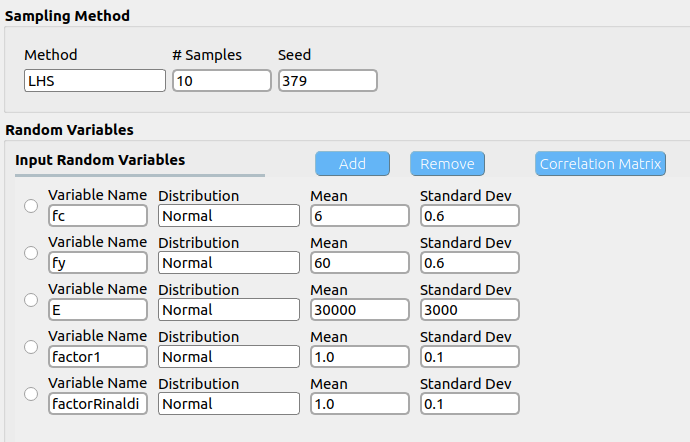
\includegraphics[width=1.0\textwidth]
    {usage/figures/uq1.png} }
  \caption{Uncertainty Quantification input panel}
  \label{fig:uq_panel}
\end{figure}

\subsection{Random Variables}
The Random Variable panel allows the user to characterize the random
variables. Each random variable has a name and a distribution. The
distribution is selected from the drop-down menu. By changing the
distribution type, the parameters required to define the distribution
change. The following distributions are available (clicking on a link will take you to the Dakota manual that provides theoretical background and explains the requested parameters for each distribution):
\begin{enumerate}
\item \href{https://dakota.sandia.gov//sites/default/files/docs/6.9/html-ref/variables-normal_uncertain.html}{Normal}
\item \href{https://dakota.sandia.gov//sites/default/files/docs/6.9/html-ref/variables-lognormal_uncertain.html}{Lognormal}
\item \href{https://dakota.sandia.gov//sites/default/files/docs/6.9/html-ref/variables-beta_uncertain.html}{Beta}
\item \href{https://dakota.sandia.gov//sites/default/files/docs/6.9/html-ref/variables-uniform_uncertain.html}{Uniform}
\item \href{https://dakota.sandia.gov//sites/default/files/docs/6.9/html-ref/variables-weibull_uncertain.html}{Weibull}
\item \href{https://dakota.sandia.gov//sites/default/files/docs/6.9/html-ref/variables-gumbel_uncertain.html}{Gumbel}
\end{enumerate} 

As with other panels, the random variables can be added or
removed. Care must be taken by the user in ensuring that if the user
removes random variables from this panel that they also remove them
from the other input widgets. Failing to do so may result in the
program failing to complete.



\subsection{Forward Propagation}
In the forward propagation problem, the user selects the sampling 
method to use from the dropdown menu \href{https://dakota.sandia.gov//sites/default/files/docs/6.9/html-ref/method-sampling.html}{sampling methods}. Currently there are five options available: 
Monte Carlo Sampling (MCS),  Latin Hypercube Sampling (LHS), Importance Sampling (IS), and sampling based on surrogate models, including Gaussian Process Regression (GPR) and Polynomial Chaos Expansion (PCE). Depending on the option selected, the user must specifies the appropriate input parameters for each. For instance, for MCS, the number of samples specifies the number of simulations to be performed, and providing a random seed allows the user to reproduce the same set of samples from the random variables multiple times.


\begin{figure}[!htbp]
  \centering {
    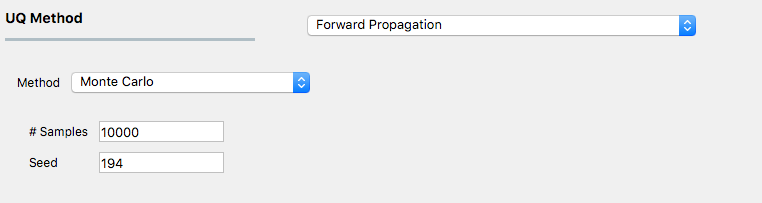
\includegraphics[width=1.0\textwidth]
    {examples/fig_quofem/fw_mc.png} }
  \caption{Monte Carlo Sampling input panel}
  \label{fig:mcs}
\end{figure}

Monte Carlo Sampling (MCS) is based on random sampling and is thus among the most robust approaches for problems where other uncertainty propagation schemes fail. Moreover, the convergence rate of MCS methods is independent of the problem dimensionality, albeit the convergence rate of such MCS methods is relatively slow $N^{-1/2}$. In MCS, a sample drawn at any step is independent of all previous samples. 

Figure \Cref{fig:mcs} shows the input panel corresponding to the Monte Carlo Sampling (MCS) setting. Two input parameters need to be specified, the number of samples to be executed, as well as the seed used in generating the random samples. 


\begin{figure}[!htbp]
  \centering {
    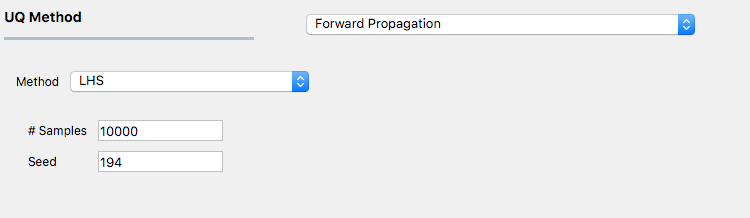
\includegraphics[width=1.0\textwidth]
    {examples/fig_quofem/fw_lhs.png} }
  \caption{Latin Hypercube Sampling input panel}
  \label{fig:lhs}
\end{figure}

Latin Hypercube Sampling (LHS) represents a pseudo-random, stratified sampling approach for uncertainty propagation. With a better convergence rate than MCS, LHS pseudo-sampling take into account all previous sample points before drawing a new sample point.  

Figure \Cref{fig:lhs} shows the input panel corresponding to the Latin Hypercube Sampling (LHS) scheme. Two input parameters also need to be specified, the number of samples to be executed, as well as the seed used in generating the LHS samples. 

\begin{figure}[!htbp]
  \centering {
    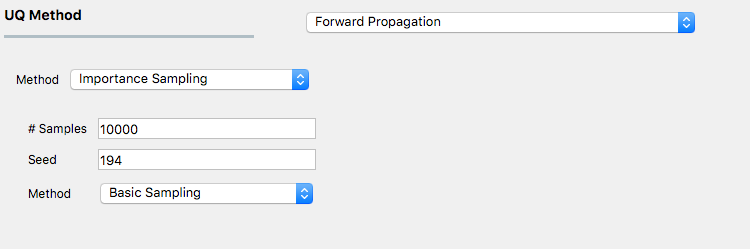
\includegraphics[width=1.0\textwidth]
    {examples/fig_quofem/fw_is.png} }
  \caption{Importance Sampling input panel}
  \label{fig:is}
\end{figure}

For problems where one is interested in the tail events rather than the distribution itself, such as rare earthquake or storm surge events, conventional sampling methods do not perform well, or might need a high number of samples to obtain an accurate estimation of tail distribution. For such problems, Importance Sampling provide a bypass to conventional sampling (LHS or MCS), whereby an alternative distribution is constructed with more weight on the tail part so that samples are concentrated there and this more accurate estimates of tail events are achieved. 

For rare event analysis, Figure \Cref{fig:is} shows the input panel for Importance Sampling (IS) scheme. Similar to MCS and LHS, the IS requires both the number of samples to be executed and the corresponding seed for generating such random samples. In addition, the Importance Sampling algorithm can performed via three different approaches, as specified by the third input method. The latter includes

\begin{enumerate}
\item Basic Sampling: a sampling density is constructed in the failure region based on an initial LHS sampling, followed by generation of importance samples and weights and evaluation of the Cumulative Distribution Function.  
\item Adaptive Sampling: similar to based sampling, with the exception that the basic sampling procedure is repeated iteratively until a convergence in failure probability is achieved. 
\item Multimodal Adaptive Sampling: a multimodal sampling density is constructed based on samples in the failure region, from which, the adaptive sampling procedure is used.
\end{enumerate}

For more information on each, please refer to the Dakota manual. 


For uncertainty propagation with surrogates, two popular surrogates are available, namely Gaussian Process Regression (GPR) and Polynomial Chaos Expansion (PCE). Figure \Cref{fig:gpr} shows the input panel for the GPR model, with input panels for training and sampling. 

\begin{figure}[!htbp]
  \centering {
    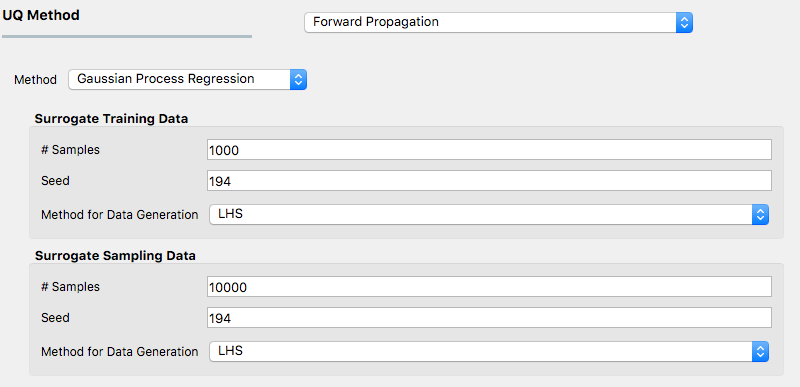
\includegraphics[width=1.0\textwidth]
    {examples/fig_quofem/fw_gp.png} }
  \caption{GPR forward propagation input panel}
  \label{fig:gpr}
\end{figure}

For problems where conventional sampling schemes such as LHS, MCS, or other fail, surrogates can be leveraged to obtain an approximation of the response surface, and than sample from that surface accordingly. 

Gaussian Process Regression, also known as Kriging, represent a well-established method for interpolation and response surface construction based on Gaussian process models with covariance matrices.  

For uncertainty propagation with Gaussian Process Regression (GPR), Figure \Cref{fig:gpr} shows the input panel for the PCE model, with input panels for training and sampling as well. The first set of input parameters in the surrogate training data specify the dataset used for training the surrogate model, while the second set of input parameters in the surrogate sampling data relate to the dataset used for sampling the surrogate. Care must be taken in specifying the training dataset to results in an accurate response surface approximation. 

\begin{figure}[!htbp]
  \centering {
    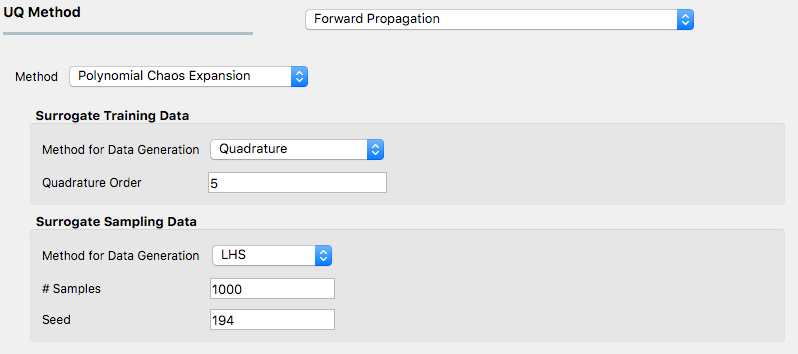
\includegraphics[width=1.0\textwidth]
    {examples/fig_quofem/fw_pce.png} }
  \caption{PCE forward propagation input panel}
  \label{fig:pce}
\end{figure}

Another response surface approximation scheme is based on Polynomial Chaos Expansion (PCE) scheme. For uncertainty propagation with Polynomial Chaos Expansion (PCE), Figure \Cref{fig:pce} shows the input panel for the PCE model, with input panels for training and sampling as well, similar to the input GPR panel. The first set of input parameters in the surrogate training data specify the dataset used for training the surrogate model, while the second set of input parameters in the surrogate sampling data relate to the dataset used for sampling the surrogate. Extreme care must be taken in specifying the parameters of the training dataset to results in an accurate response surface approximation. 

If you are not sure about the training parameters of the surrogates, please refrain from using the surrogates (PCE in particular) for forward propagation and use instead conventional sampling such as MCS and LHS as discussed above, 
even at a higher computational cost. 

\subsection{Reliability Analysis}

For reliability analysis, first-order (FORM) and second-order (SORM) methods represent two popular, well-established, robust methods. For a First-Order Reliability Method (FORM), the performance function is approximated by a first order Taylor expansion, while for a second-order expansion using for SORM. 

Methods, moreover, for both global and local reliability analysis have emerged over the past decades and are, to a varying degree, well-established. 

For reliability analysis, figure \Cref{fig:rel} shows the input panel for the reliability capabilities. Currently, both First-Order Reliability Methods (FORM) and Second-Order Reliability Methods (SORM) are supported. The user can specify the local or global solution in the Reliability Scheme input parameter. In addition, the user needs to specify the method for searching for the Most Probable Point (MPP); if not sure, do not use any MPP approximation. 

For both first and second-order reliability analysis, the user needs to specify the either the response levels or the probability levels at which the CDF of the QoI needs to be queried. The user can specify multiple query points, separated by a space. 


\begin{figure}[!htbp]
  \centering {
    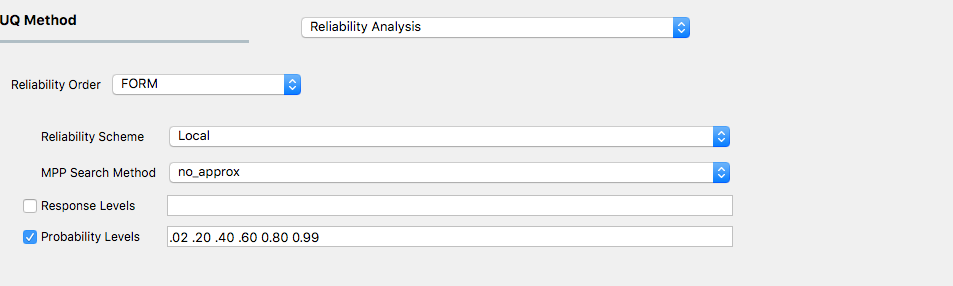
\includegraphics[width=1.0\textwidth]
    {examples/fig_quofem/rel_form.png} }
  \caption{Reliability input panel}
  \label{fig:rel}
\end{figure}


\subsection{Inverse Problem}


For the Inverse problem following a Bayesian updating paradigm, a prior distribution on a parameter is updated through a Bayesian framework involving experimental data and a likelihood function. In Bayesian methods, uncertain parameters are characterized by probability density functions. These probability density functions define the permissible parameter values the support, as well as the relative plausibility of each permissible parameter value. In the context of calibration or any inference step, the probability density function that describes knowledge before the incorporation of data is called the prior. When data are available, the likelihood function describes how well each parameter value is supported by the data. Bayes Theorem is used for inference: to derive the plausible parameter values, based on the prior probability density and the data. The result is the posterior probability density function of the parameters. It is interpreted the same way as the prior, but includes the information derived from the data.


\textbf{DREAM}: This is popularly known as DiffeRential Evolution Adaptive Metropolis (DREAM) algorithm [9, 10] for Bayesian estimation. The DREAM method allows the user to define the number of chains used with the chains specification. The total number of generations per chain in DREAM is the number of samples divided by the number of chains. The number of chains randomly selected to be used in the crossover each time a crossover occurs is crossover chain pairs. There is an extra adaptation during burn-in, in which DREAM estimates a distribution of crossover probabilities that favors large jumps over smaller ones in each of the chains. Normalization is required to ensure that all of the input dimensions contribute equally. In this process, a discrete number of candidate points for each crossover value are generated, which can be specified. The threshold control is the convergence tolerance for the Gelman-Rubin statistic, which governs the convergence of the multiple chain process. The integer jump step forces a long jump for every jump step generated. Credible and prediction intervals can be calculated by specifying probability levels, and statistics regarding the posterior may be calculated by specifying posterior stats.

Figure \Cref{fig:inv} shows the input panel corresponding to the inverse analysis module. Currently, only the DREAM method, is supported. For the DREAM method, the user needs to specify the number of Markov chain iterations to use for the method. Other data assimilation methods are currently being implemented and will be part of the upcoming releases. 


\begin{figure}[!htbp]
  \centering {
    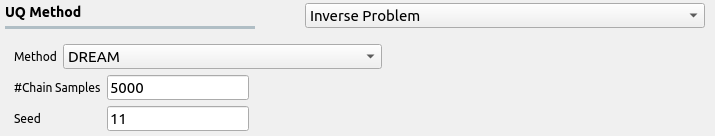
\includegraphics[width=1.0\textwidth]
    {examples/fig_quofem/inv_dream.png} }
  \caption{Inverse problem input panel}
  \label{fig:inv}
\end{figure}

\subsection{Parameter Estimation}

For parameter estimation, figure \Cref{fig:pe} a typical input panel. Two different optimization algorithms are currently provided, namely OPT++GaussNewton NL2SOL. A description of these algorithms can be found in Dakota. Two input parameters need to be specified for estimation, the convergence tolerance and the maximum number of iterations of the optimization subroutine. 

\begin{figure}[!htbp]
  \centering {
    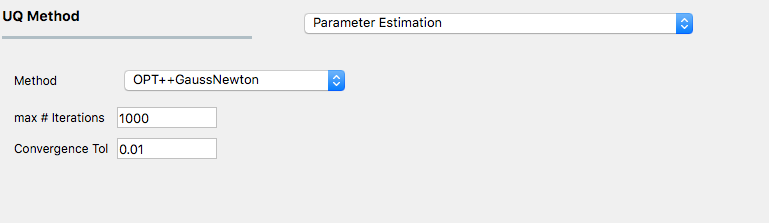
\includegraphics[width=1.0\textwidth]
    {examples/fig_quofem/param_est.png} }
  \caption{Parameter estimation input panel}
  \label{fig:pe}
\end{figure}


\subsection{Global Sensitivity Analysis}

For the Global Sensitivity Analysis problem, a typical input panel is shown in figure \Cref{fig:sens}. In the current implementation, a global approximation of the response surface is performed using conventional sampling. 

The global sensitivity analysis produces two indices, namely main and total indices. For a detailed description of these global indices, please refer to the Dakota manual. 

\begin{figure}[!htbp]
  \centering {
    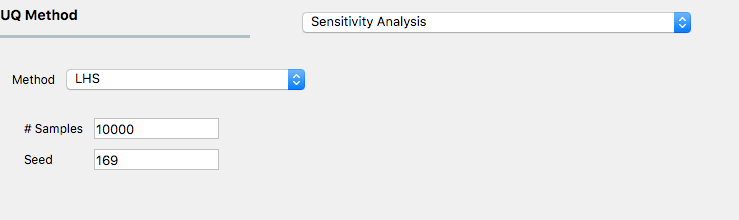
\includegraphics[width=1.0\textwidth]
    {examples/fig_quofem/sens.png} }
  \caption{Sensitivity analysis input panel}
  \label{fig:sens}
\end{figure}




